% This is based on samplepaper.tex, LLNCS macro package for Springer
\documentclass[runningheads]{llncs}

% Language & Encoding
\usepackage[T1]{fontenc}
\usepackage[utf8]{inputenc} 
\usepackage[english]{babel}

% Math Symbols
\usepackage{amsmath}
\usepackage{amsfonts}
\usepackage{amssymb}

% Graphics & Utils
\usepackage{graphicx}
\graphicspath{{img/}}
\usepackage{float} % Helps with floating graphics and tables

% Hyperlinks
\usepackage{hyperref}
\usepackage{color}
\renewcommand\UrlFont{\color{blue}\rmfamily}
\urlstyle{rm}

\begin{document}

% Metadata
\title{Comparative Analysis of Solutions for the Traveling Salesman Problem (TSP)}

% Appears in even pages' headers
\titlerunning{Analysis of TSP Algorithms}

% Author Names (Same University)
\author{Daniel-Ioan Dinu \inst{1} \and
Maria-Ioana Ungurean \inst{1} \and
Mihai Toderiță \inst{1}}

% Appears in odd pages' headers
\authorrunning{D. Dinu, M. Ungurean, M. Toderiță} 

% Institute & Emails
\institute{National University of Science and Technology Politehnica Bucharest\\
Faculty of Automatic Control and Computers\\
\email{\{daniel\_ioan.dinu, maria.ungurean, mihai.toderita\}@stud.acs.upb.ro}}

\maketitle

% Abstract
\begin{abstract}
This report presents a comparative analysis of three algorithms for solving the Traveling Salesman Problem (TSP): Brute Force, Greedy (Nearest Neighbor), and Held-Karp. The study evaluates time performance and solution accuracy on a set of 25 synthetic tests.

\keywords{Traveling Salesman Problem \and Algorithms \and Benchmarking.}
\end{abstract}

% Content Sections

\section{Introduction}
\label{sec:intro}

\subsection{Problem Description}

The Traveling Salesman Problem (TSP) represents one of the most studied problems in combinatorial optimization, appealing greatly to modern 
logistics. The problem statement is deceptively simple: given a list of cities and the distances between any pair of cities, what is the 
shortest possible route that visits each city exactly once and returns to the origin city? Several algorithms have come up across decades, some 
that guarantee an optimal solution for smaller problems, while others produce near-optimal answers fast enough for real-life applications.

Formally, the problem is defined on a weighted complete graph $G = (V, E, w)$, where $V$ is the set of nodes (cities), $E$ is the 
set of edges, and $w: E \to \mathbb{R}^+$ is the cost function. The objective is to find a permutation $\sigma$ of the nodes that 
minimizes the sum:

\begin{equation}
    Cost = \sum_{i=1}^{n-1} w(v_{\sigma(i)}, v_{\sigma(i+1)}) + w(v_{\sigma(n)}, v_{\sigma(1)})
\end{equation}

\subsection{Real-life Applications}

Studying TSP has direct implications for clever logistics and transportation: even tiny improvements worth a few kilometers saved daily will 
contribute to big savings across vehicle fleets, interconnected warehouses, and regional networks. Its computational complexity, on the other 
hand, demonstrates that real applications won't use TSP as is. The preferred strategy is a combination of more adaptations of TSP: Multiple 
Salesmen Problem (mTSP), TSP with Time Windows (TSPTW), Time-dependent TSP, Dynamic TSP \cite{tsp_adaptations}. 
Other applications of TSP and its adaptations include: X-Ray crystallography, computer wiring, mask plotting in PCB production and printing 
press scheduling. \cite{matai2010traveling}

hello from NP Hard demonstration

\section{Descrierea Algoritmilor Implementați}
\label{sec:algoritmi}

În această secțiune detaliem implementarea celor trei algoritmi utilizați în cadrul studiului comparativ, evidențiind modul în care aceștia gestionează cazurile particulare (grafuri rare) și constrângerile de memorie.

\subsection{Brute Force (Căutare Exhaustivă)}
Implementarea utilizează funcția \texttt{std::next\_permutation} din biblioteca standard C++ pentru a genera sistematic toate rutele posibile.

\begin{itemize}
    \item \textbf{Mod de lucru:} Algoritmul fixează nodul $0$ ca punct de start și generează toate permutările celorlalte $n-1$ noduri.
    \item \textbf{Gestiunea erorilor:} Pentru a preveni erorile de tip \textit{overflow}, am utilizat o constantă \texttt{SAFE\_INT}. Dacă o muchie lipsește sau drumul este invalid, costul este setat la această valoare, iar suma nu este incrementată peste limită.
    \item \textbf{Complexitate:} $O(n!)$, fiind limitat de numărul total de permutări.
\end{itemize}

\subsection{Held-Karp (Programare Dinamică și Bitmasking)}
Algoritmul Held-Karp reprezintă o optimizare semnificativă, reducând spațiul de căutare prin memorarea rezultatelor parțiale.

\begin{itemize}
    \item \textbf{Structuri de date:} Am utilizat un tabel DP de tip \texttt{std::vector<std::vector<int>>} de dimensiune $n \times 2^n$. 
    \item \textbf{Bitmasking:} Starea subproblemelor este reprezentată printr-un întreg (\texttt{mask}), unde al $i$-lea bit este $1$ dacă orașul $i$ a fost vizitat și $0$ în caz contrar.
    \item \textbf{Recursivitate:} Funcția \texttt{totalCost} calculează recursiv drumul minim, verificând la fiecare pas dacă drumul rămas este valid (\texttt{remaining < SAFE\_INT}) înainte de a actualiza optimul local.
\end{itemize}



\subsection{Greedy (Nearest Neighbour)}
Este cel mai rapid algoritm implementat, având o abordare constructivă, bazată pe alegeri locale.

\begin{itemize}
    \item \textbf{Logică:} La fiecare pas, algoritmul caută în matricea de adiacență cel mai apropiat vecin nevizitat al orașului curent.
    \item \textbf{Eșec Structural (Dead End):} Codul implementat tratează explicit cazul în care nu există muchii către orașe nevizitate. În această situație, algoritmul returnează \texttt{SAFE\_INT}, semnalând imposibilitatea finalizării turului (fapt confirmat de rezultatele din Tabelul \ref{tab:accuracy}).
    \item \textbf{Complexitate:} $O(n^2)$, datorită celor două bucle imbricate necesare pentru vizitarea a $n$ orașe și căutarea vecinului minim.
\end{itemize}
\section{Evaluation}
\label{sec:evaluation}

For the three previously described algorithms, we performed a complete analysis of both solution accuracy and time performance. In order to 
achieve this, we constructed a diverse set of tests which covers different sizes and densities that input graphs for TSP might have. Since 
all graphs that are meant to have an answer to TSP are complete and weighted at the same time, this narrows down the edge cases significantly.

%% 1. Construction of the Test Set %%
\subsection{Construction of the Test Set}
\label{subsec:tests}

To ensure a rigorous validation of the three algorithms, we developed a synthetic benchmark generator designed to produce instances of varying difficulty. The methodology relies on a controlled scaling of the input size ($N$) and a stochastic variation of graph density. The test set comprises 25 instances, categorized into three distinct difficulty tiers:

\begin{enumerate}
    \item \textbf{Small-Scale Instances ($N \in [3, 10]$):} Primarily used to verify the correctness of the Brute Force implementation and to establish a baseline for solution accuracy.
    \item \textbf{Medium-Scale Instances ($N \in [11, 18]$):} Designed to observe the exponential growth of the Brute Force algorithm and the transition of Held-Karp into its primary operational range.
    \item \textbf{Limit-Testing Instances ($N \in [19, 20]$):} These instances push the computational limits of exact algorithms, particularly Held-Karp, highlighting the efficiency of dynamic programming over exhaustive search.
\end{enumerate}

The graph topology for each test is generated by first considering a complete graph $K_n$ and then performing a random edge-pruning process. The number of edges $M$ is selected such that $n \le M \le \frac{n(n-1)}{2}$, ensuring that the graph remains potentially Hamiltonian while varying in density. This approach allows us to test the Greedy heuristic's robustness in "sparse" environments, where the lack of backtracking may lead to a failure in finding a valid Hamiltonian cycle. Edge weights are assigned as uniform integers in the range $[1, 10^6]$ to prevent trivial solutions and test for potential integer overflow handling.

%% 2. Computing System Specifications %%
\subsection{Computing System Specifications}
\label{subsec:specs}

We ran all experiments on a native Linux system belonging to one of the team members to eliminate overhead caused by virtual machines or WSL. 
The hardware and software configuration used for benchmarking was as follows:

\begin{itemize}
    \item Operating System: EndeavourOS x86\_64 (Linux Kernel 6.12.63-1-lts)
    \item Processor: Intel Core Ultra 5 125U (14 cores, max frequency 4.30 GHz)
    \item RAM: 32 GB (30.82 GiB usable)
    \item Compiler: g++ (GCC) 15.2.1 20251112, no optimization
    \item Framework: Google Benchmark \cite{googlebenchmark} v1.8.3
\end{itemize}

%% 3. Illustration of Results %%
\subsection{Illustration of Results}
\label{subsec:illustration}

We ran the benchmark on the Test Set for a total of 20 times, in order to have a large enough sample size. For this subsection, we will present one of these 
runs, taking a closer look at the individual test results, then proceed to formulate a statistic featuring the average computation time for every test 
and the average error caused by the Greedy approach. It is important to note that running the benchmark back-to-back 20 times generate a lot of heat, 
causing the processor to adjust. The benchmarking itself is a CPU-bound task to solve. This way, the single instance study should provide a clear view 
on the rae performance and precision of the algorithms, while the statistic offers the more realistic, scalable view.

\subsubsection{Qualitative Analysis on One Benchmark Run}

The chosen sample (Table \ref{tab:benchmark_summary}) confirms the differences in complexity classes among the algorithms: one that quickly reaches 
impractical runtime, another that exhibits significant growth with complex input data, and one that remains predictable.

\begin{table}[H]
    \centering
    \caption{Example of execution times measured on one run of all tests.}
    \label{tab:benchmark_summary}
    \begin{tabular}{|l|c|r|r|r|}
        \hline
        \textbf{Test} & \textbf{Node Count} & \textbf{Brute Force} & \textbf{Held-Karp} & \textbf{Greedy} \\
        \hline
        Test 08 & 4  & 44 ns            & 84 ns             & 18 ns \\
        Test 01 & 8  & 22.5 $\mu$s      & 3.9 $\mu$s        & 56 ns \\
        Test 09 & 10 & 2.22 ms          & 75 $\mu$s         & 85 ns \\
        Test 12 & 12 & 248 ms           & 0.51 ms           & 120 ns \\
        Test 11 & 13 & \textbf{1.63 s}  & 0.64 ms           & 130 ns \\
        Test 18 & 14 & \textit{Timeout} & 3.11 ms           & 162 ns \\
        Test 19 & 17 & \textit{Timeout} & 35.6 ms           & 238 ns \\
        Test 24 & 20 & \textit{Timeout} & \textbf{644 ms}   & 328 ns \\
        \hline
    \end{tabular}
\end{table}

In addition to execution time, a factor we considered in evaluating the algorithms is the correctness of the obtained solution. Table 
\ref{tab:accuracy} compares the path cost found by the Greedy heuristic with the optimal cost calculated by Held-Karp. We noticed how far 
the Greedy algorithm can deviate from the real solution, often exceeding the \textit{SAFEINT} constant used in our study to signal a run failure. 
We distinguish three situations that can occur:

\begin{itemize}
    \item Rare Success: In isolated cases (e.g., Test 08), the local choice coincides with the global optimum \textbf{at every step}, resulting in a 0\% error.
    The graph for this test is a sparse graph with 4 nodes and 5 edges, which looks geometrically like two triangles sharing a common side.
    \item Cascading Deviations: In most successful cases, Greedy produced solutions with a visibly higher cost than the optimal one. 
    This is due to a choice that respects the heuristic but, overall, disqualifies a part of the optimal solution from being considered. 
    A "snowball effect" can occur, amplifying the discrepancies.
    \item General Failure: Since the Nearest Neighbor algorithm has no backtracking mechanism, if it reaches a node from which it can no 
    longer visit the remaining cities (such as in a sparse graph), execution blocks.
\end{itemize}

\begin{table}[H]
    \centering
    \caption{Comparison of costs and relative errors on one run of all tests.} 
    \label{tab:accuracy}
    \begin{tabular}{|l|r|r|r|l|}
        \hline
        \textbf{Test} & \textbf{Optimal Cost} & \textbf{Greedy Cost} & \textbf{Error (\%)} & \textbf{Conclusion} \\
        \hline
        Test 08 & 1,248,907 & 1,248,907      & \textbf{0.00\%}  & Solution Found \\
        Test 02 & 3,077,161 & 3,123,942      & 1.52\%           & Good \\
        Test 04 & 1,501,515 & 1,665,081      & 10.89\%          & Average \\
        Test 22 & 1,645,079 & 2,456,555      & 49.33\%          & Poor \\
        Test 01 & 1,273,944 & 2,280,130      & 78.98\%          & Very Poor \\
        \hline
        Test 05 & 3,411,545 & $\infty$ (INF) & N/A              & Greedy Failed \\
        Test 11 & 5,050,651 & $\infty$ (INF) & N/A              & Greedy Failed \\
        Test 24 & 2,721,940 & $\infty$ (INF) & N/A              & Greedy Failed \\
        \hline
        Test 06 & $\infty$ (INF) & $\infty$ (INF) & N/A         & Disconnected Graph \\
        \hline
    \end{tabular}
\end{table}

From the interpretations above, we can distinguish several reasons why the discussed implementations might fail, for various situations:

\begin{itemize}
    \item \textbf{Brute Force:} Reaches its practical limit at $N \ge 13$. The failure is caused by the factorial time complexity ($O(N!)$), which inevitably leads to a \textit{Timeout}.
    \item \textbf{Held-Karp:} We estimate the limit to be around $N > 22$. Unlike Brute Force, the bottleneck here is usually \textit{Memory} ($O(N \cdot 2^N)$) rather than raw CPU time.  
    \item \textbf{Greedy:} Fails unpredictably depending on the \textit{Graph Topology}. Because the heuristic has no backtracking mechanism, it can get stuck in a node with no unvisited neighbours in sparse graphs, 
    resulting in a complete solution failure (Deadlock).
\end{itemize}

\subsubsection{Graphical Analysis on One Benchmark Run}

Using the same selected sample, we graphically illustrated comparisons between the algorithms. In Fig.~\ref{fig:runtime_all}, the logarithmic scale highlights the class 
difference between algorithms. Brute Force becomes vertical at $N=13$, when we expect it to start exceeding reasonable runtime. In contrast, Greedy stays consistently at the base of the graph.

\begin{figure}[H]
    \centering
    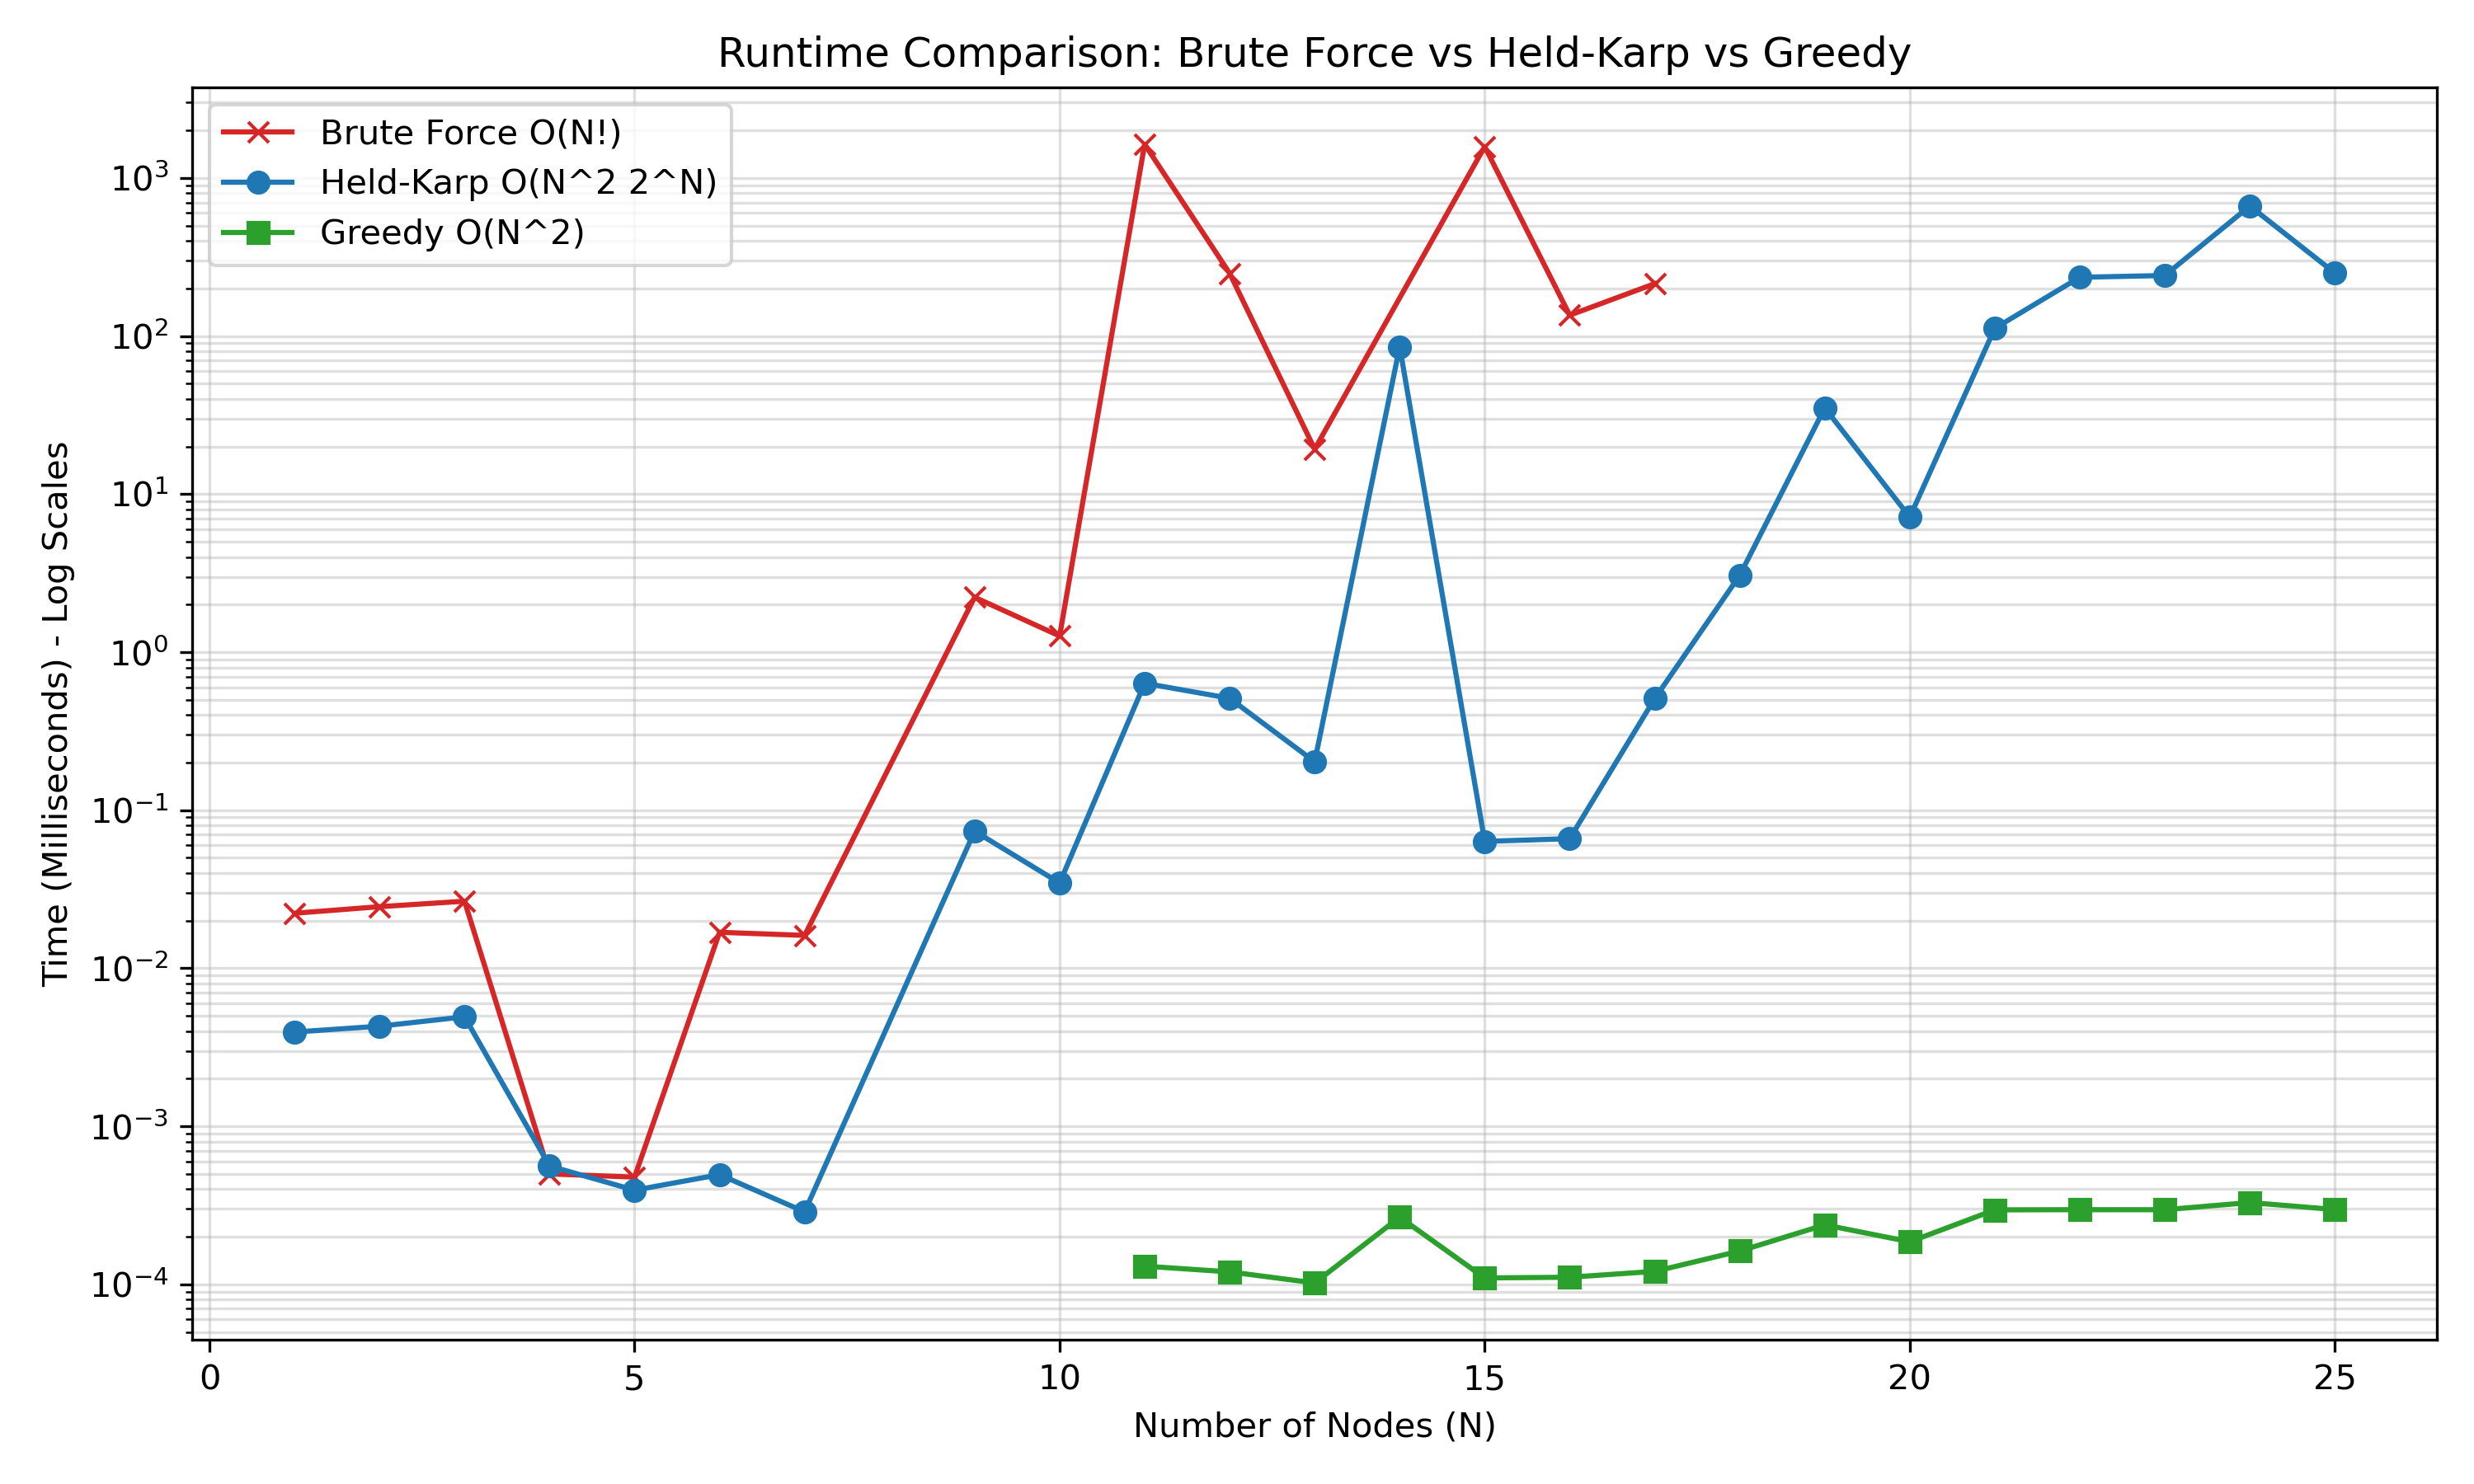
\includegraphics[width=1.0\textwidth]{plot_runtime_all.png}
    \caption{Runtime Comparison (Logarithmic Scale)}
    \label{fig:runtime_all}
\end{figure}

Although Held-Karp is much more efficient than Brute Force, Fig.~\ref{fig:hk_zoom} shows that it also follows an exponential curve, with costs 
rising rapidly after $N=17$.

\begin{figure}[H]
    \centering
    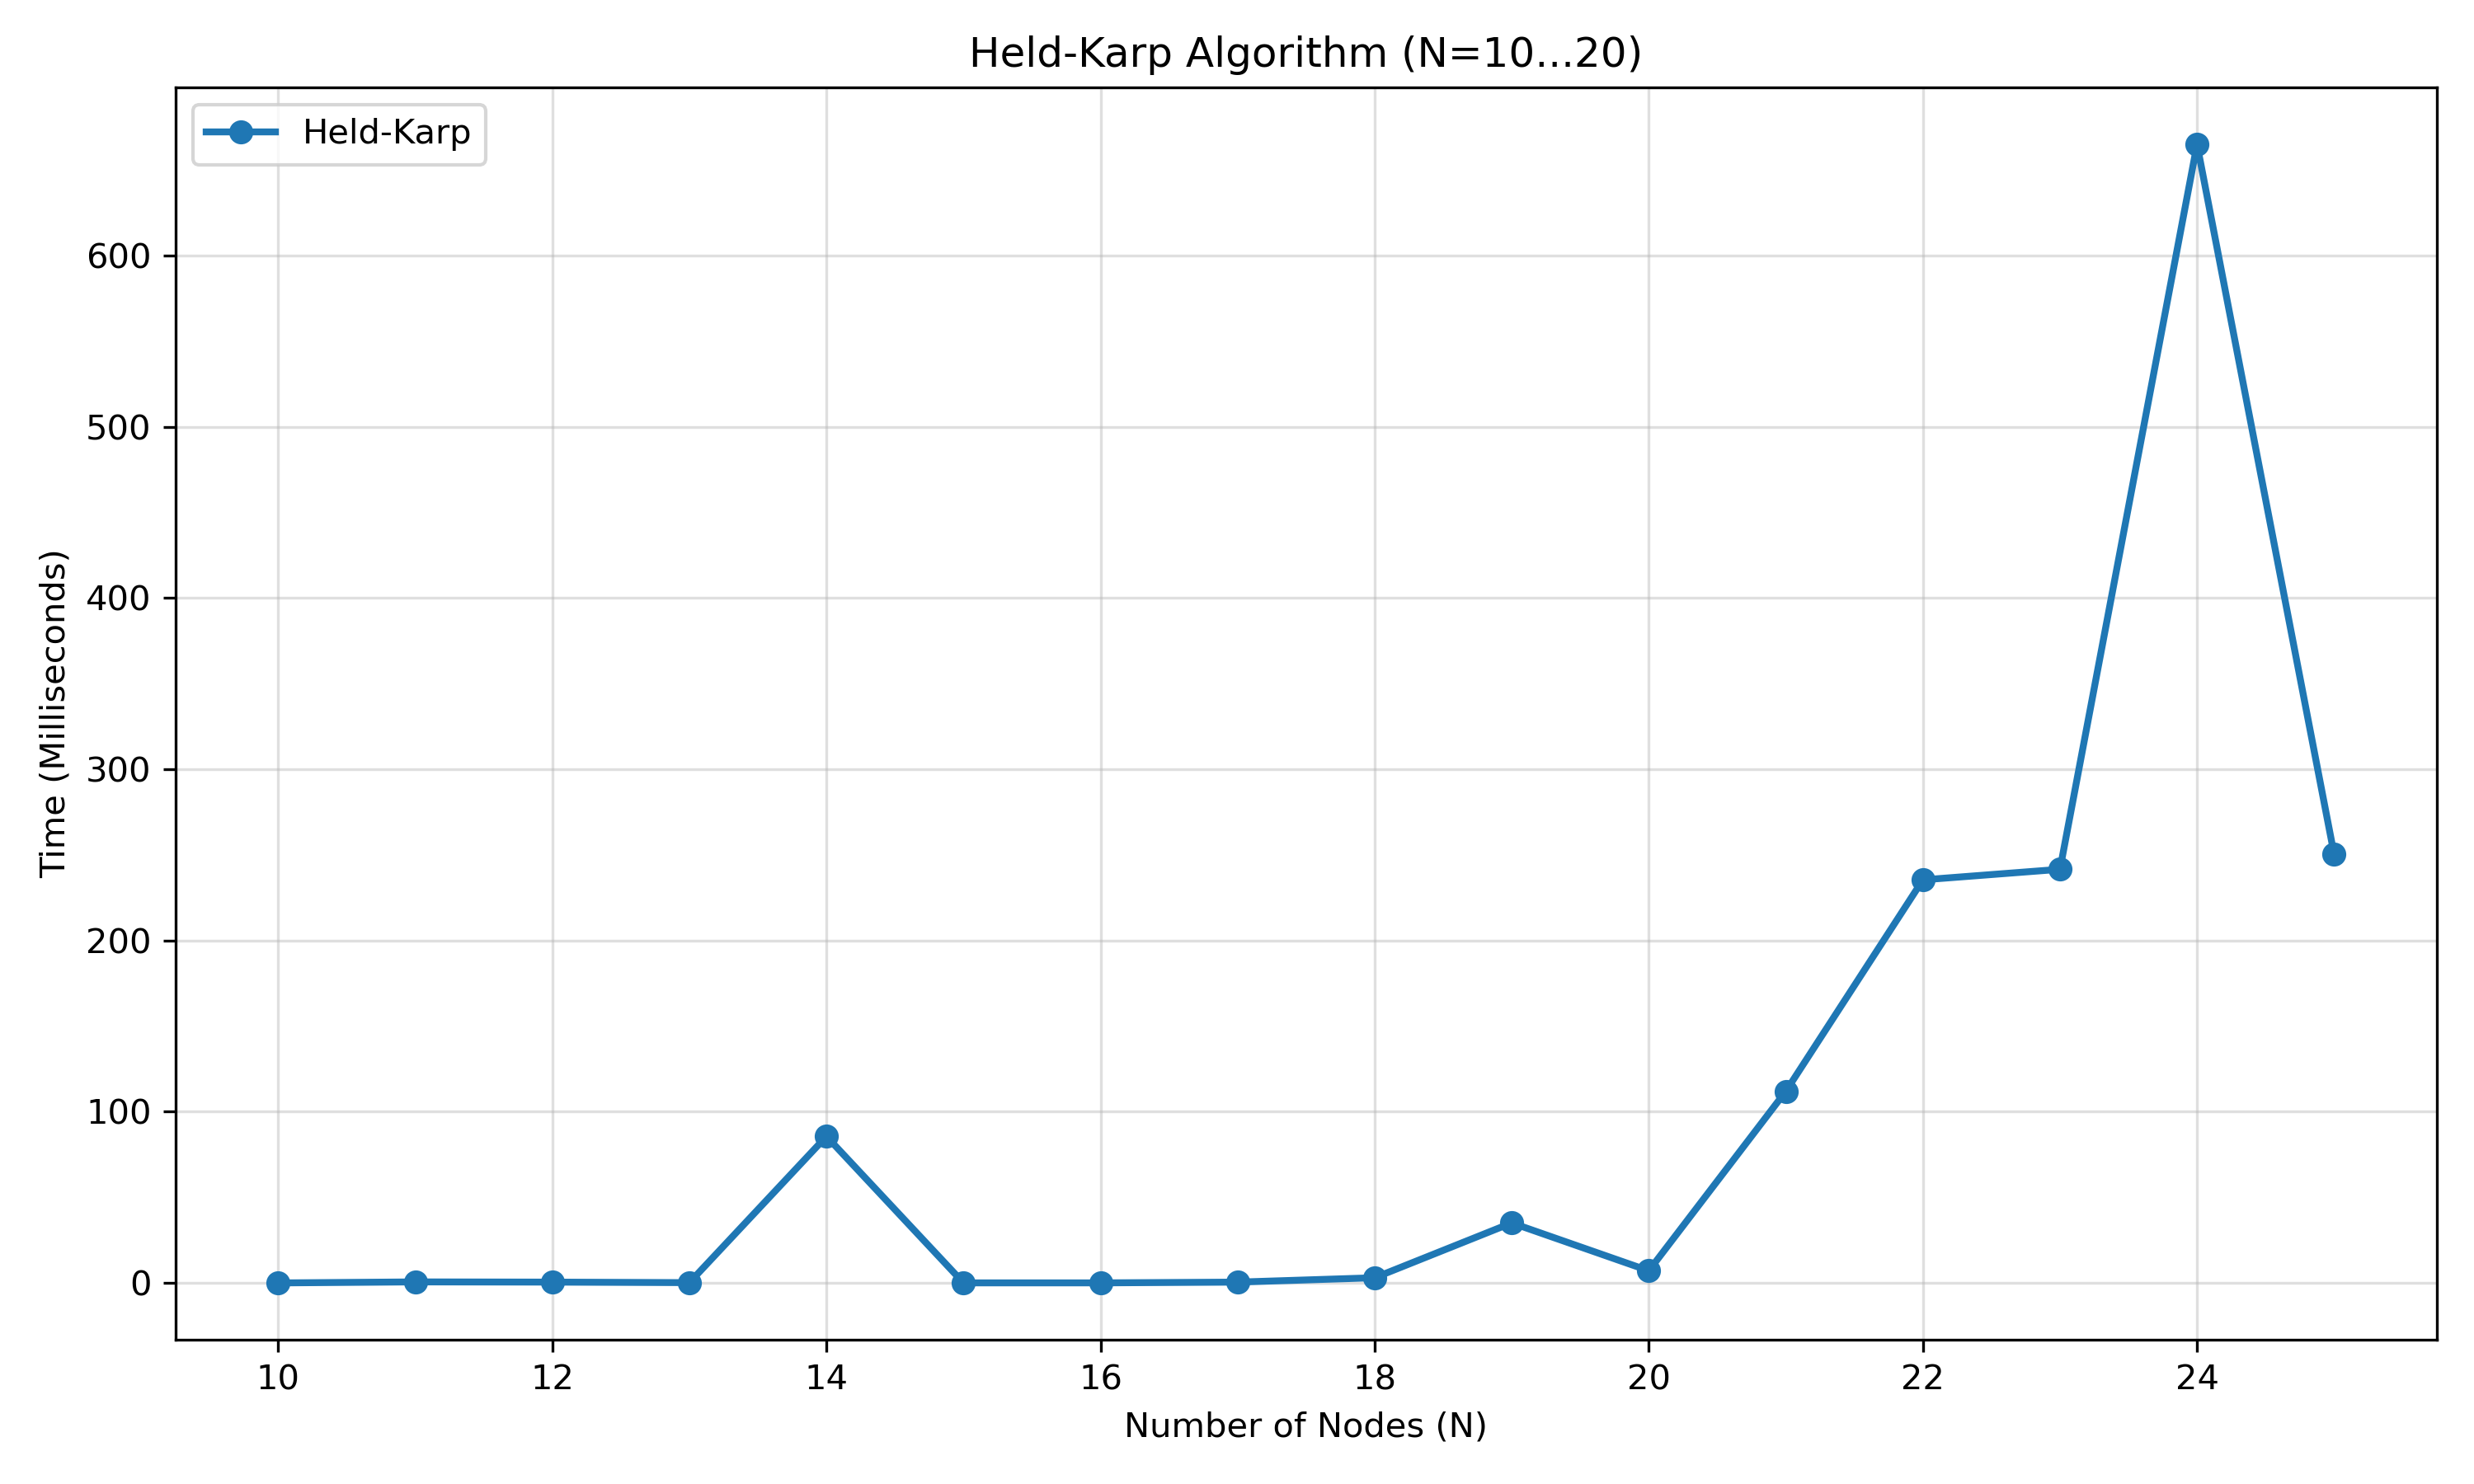
\includegraphics[width=1.0\textwidth]{plot_heldkarp_zoom.png}
    \caption{Held-Karp Performance Detail ($N=10$ to $N=20$).}
    \label{fig:hk_zoom}
\end{figure}

Finally, Fig.~\ref{fig:greedy_error} highlights the trade-off made by Greedy: maximum speed at the price of an error that reached as high 
as 80\% in our tests.

\begin{figure}[H]
    \centering
    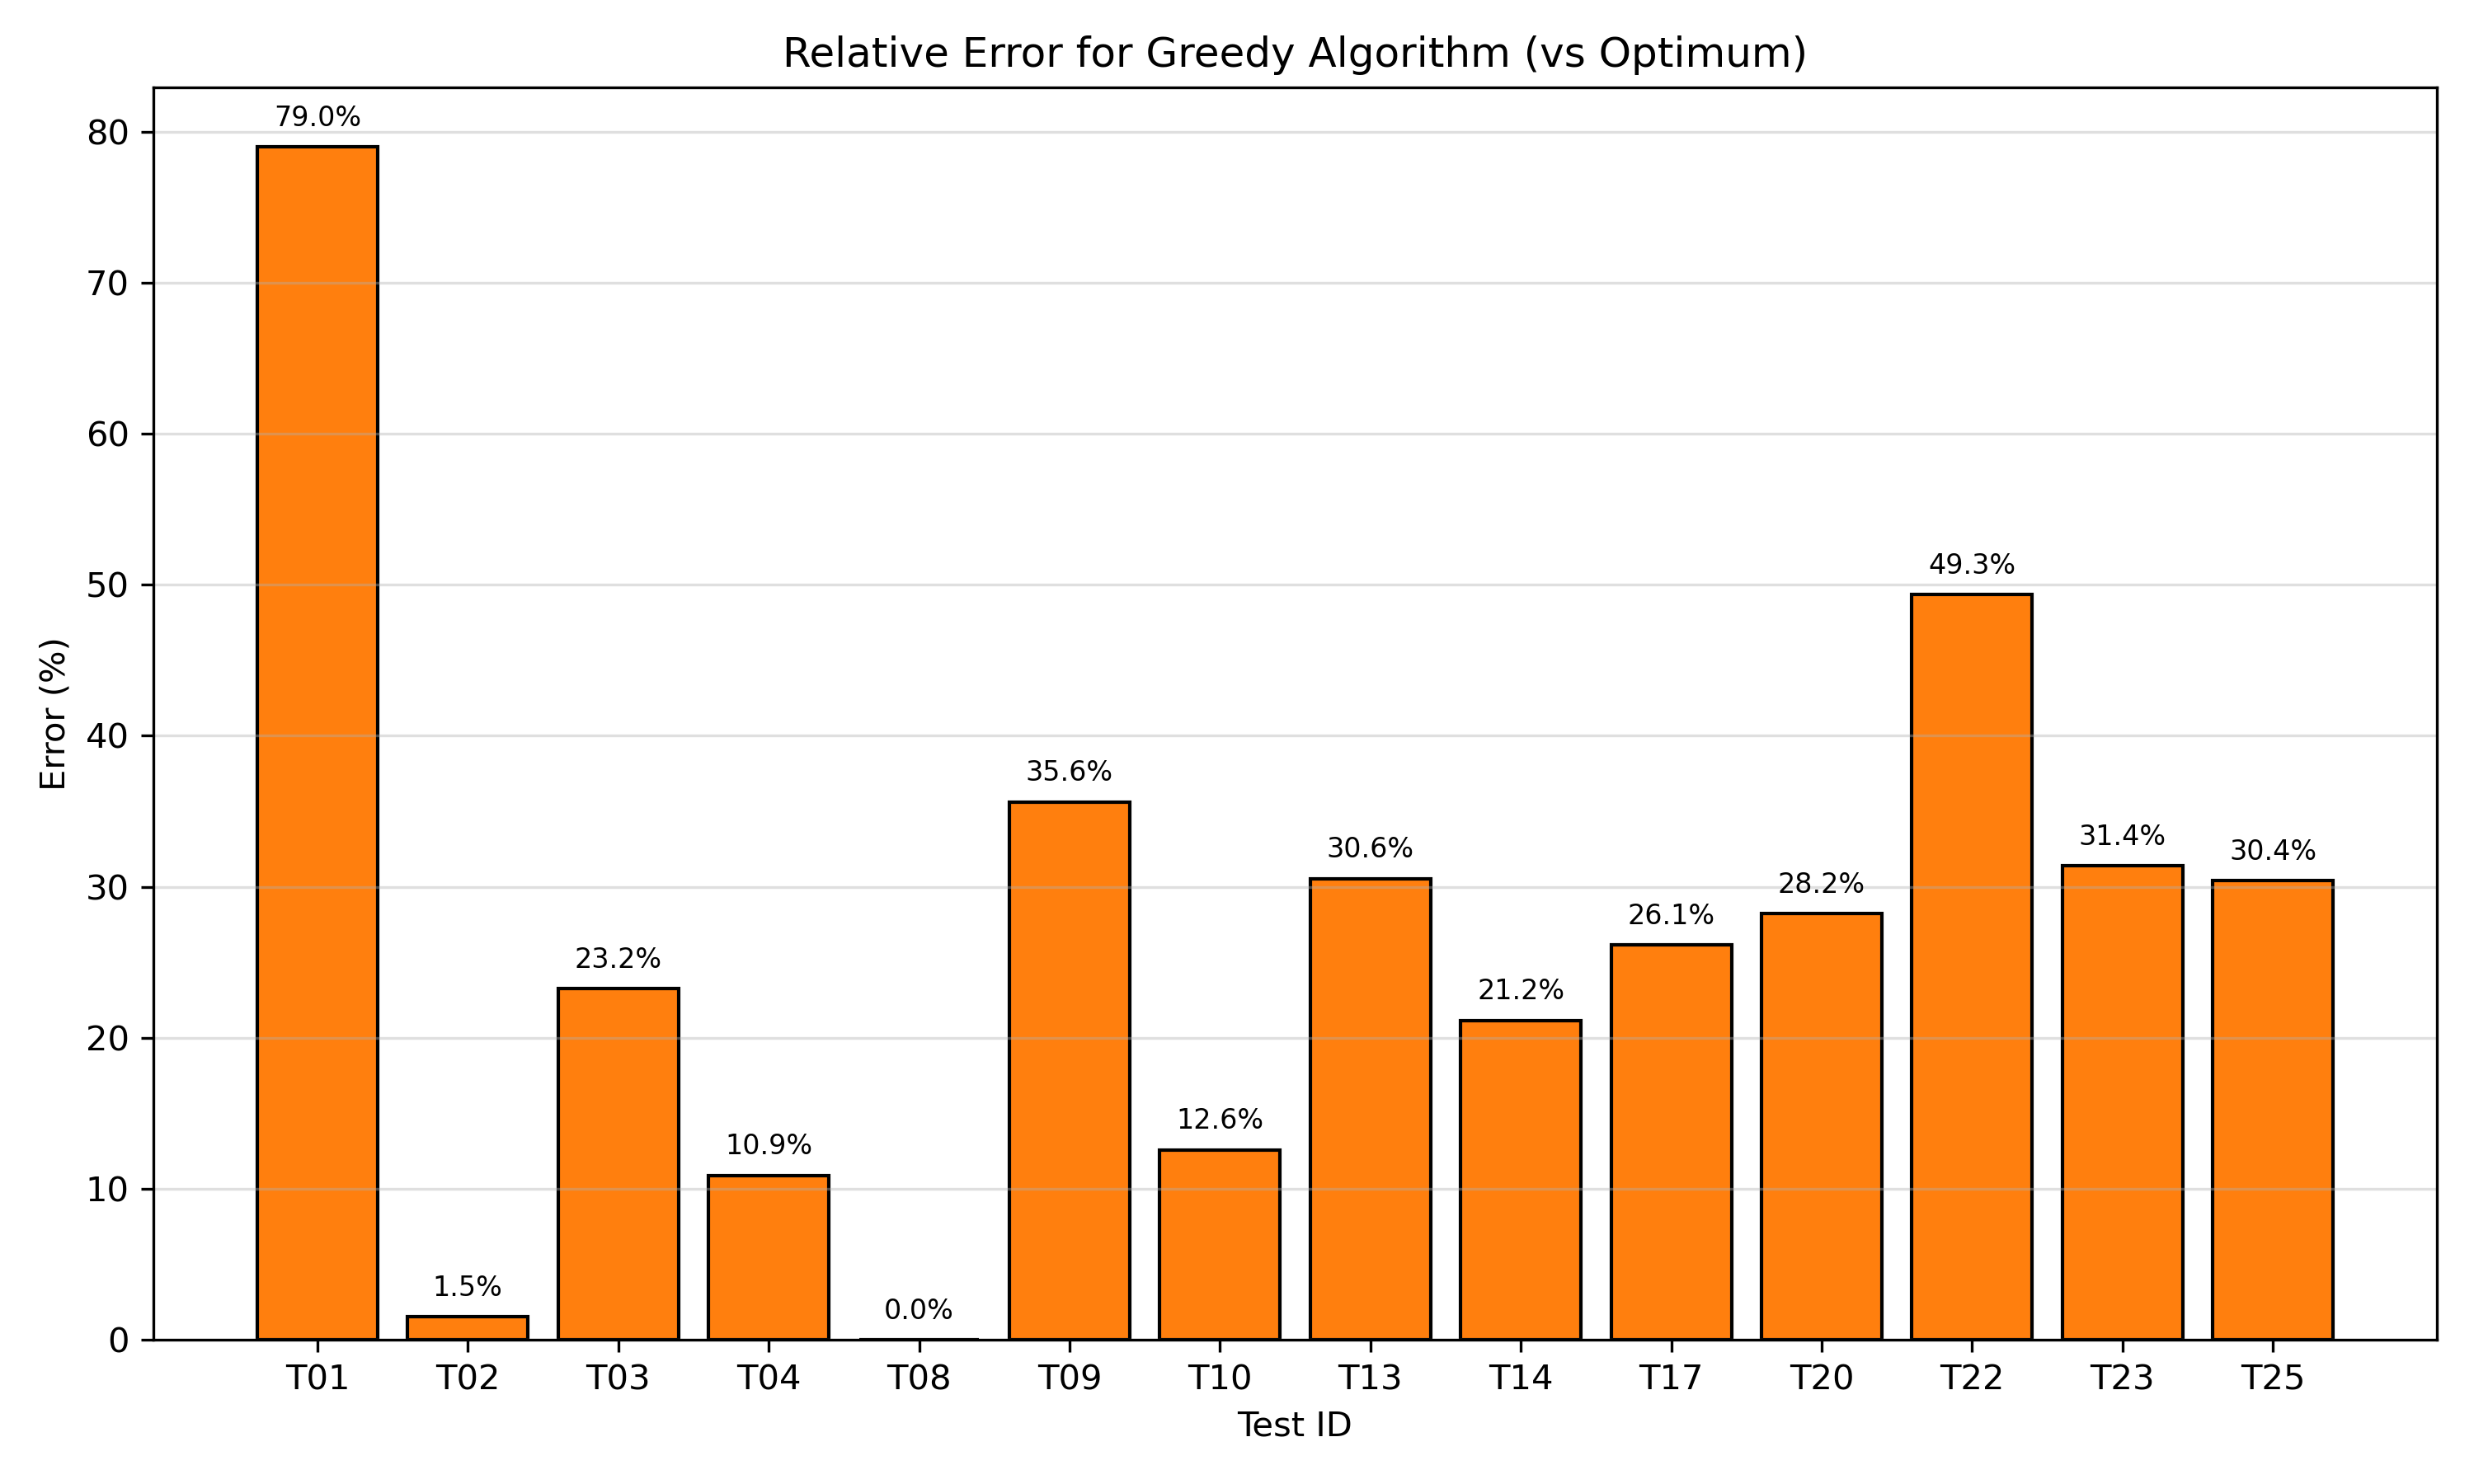
\includegraphics[width=1.0\textwidth]{plot_greedy_error.png}
    \caption{Distribution of relative errors for valid Greedy solutions.}
    \label{fig:greedy_error}
\end{figure}

%% 4. Interpretation of Results %%
\subsection{Interpretation of Results}
\label{subsec:interpretation}

\subsubsection{Overall Statistic}

Table \ref{tab:benchmark_stats} contains the simple statistic, presenting the arithmetic mean and standard deviation ($\sigma$) for these runs.

\begin{table}[H]
    \centering
    \scriptsize 
    \caption{Performance Statistics (Mean over 20 runs $\pm$ Standard Deviation).}
    \label{tab:benchmark_stats}
    \begin{tabular}{|l|c|r|r|r|r|}
        \hline
        \textbf{Test} & \textbf{N} & \textbf{Brute Force} & \textbf{Held-Karp} & \textbf{Greedy (Time)} & \textbf{Greedy (Error)} \\
        \hline
        Test 08 & 4  & 43 ns $\pm$ 0 ns             & 80 ns $\pm$ 0 ns              & 18 ns $\pm$ 0 ns    & \textbf{0.00\%} \\
        Test 04 & 6  & 499 ns $\pm$ 2 ns            & 549 ns $\pm$ 64 ns            & 34 ns $\pm$ 0 ns    & 10.89\% \\
        Test 01 & 8  & 22.5 $\mu$s $\pm$ 0.0 $\mu$s & 4.1 $\mu$s $\pm$ 0.8 $\mu$s   & 56 ns $\pm$ 0 ns    & 78.98\% \\
        Test 02 & 8  & 25.2 $\mu$s $\pm$ 2.7 $\mu$s & 4.3 $\mu$s $\pm$ 0.0 $\mu$s   & 58 ns $\pm$ 9 ns    & 1.52\% \\
        Test 09 & 10 & 2.29 ms $\pm$ 0.25 ms        & 73.5 $\mu$s $\pm$ 0.1 $\mu$s  & 89 ns $\pm$ 10 ns   & 35.62\% \\
        Test 11 & 13 & \textbf{1.68 s $\pm$ 0.08 s} & 0.64 ms $\pm$ 0.00 ms         & 130 ns $\pm$ 0 ns   & \textbf{Failed} \\
        Test 18 & 14 & \textit{Timeout}             & 3.09 ms $\pm$ 0.02 ms         & 171 ns $\pm$ 22 ns  & 26.00\% \\
        Test 24 & 20 & \textit{Timeout}             & \textbf{1.16 s $\pm$ 0.03 s}  & 328 ns $\pm$ 0 ns   & \textbf{Failed} \\
        \hline
    \end{tabular}
\end{table}

\subsubsection{Brute Force Algorithm Results}

As stated in the description of the Brute Force algorithm, its complexity is on the order of the factorial of the graph's node count ($N$). 
The increase in execution time is abrupt, and once we pass a threshold value of $N$, the algorithm reaches its practical limits. 
For example:

\begin{itemize}
    \item At $N=10$, the time is acceptable: $2.2$ ms.
    \item At $N=12$, the time increases greatly, reaching $248$ ms.
    \item At $N=13$, the algorithm takes $1.63$ seconds.
\end{itemize}

For $N \ge 14$, the time exceeded tens of seconds, even minutes, which is why we modified the benchmarking code to directly throw a runtime 
error and avoid overloading the processor.

\subsubsection{Held-Karp Algorithm Results}

The dynamic programming algorithm was able, on one hand, to manage the large volume of input data (including for node count $N=20$), and on 
the other hand, to determine the problem's answer within an acceptable execution time:

\begin{itemize}
    \item For $N=13$, Held-Karp ran in $0.63$ ms — an acceleration of \textbf{2500x} compared to Brute Force.
    \item For much larger instances, such as $N=20$, the time does not exceed one second.
\end{itemize}

However, the exponential component ($O(N^2 \cdot 2^N)$) makes its presence felt in the final tests: doubling $N$ from 10 to 20 led to an 
increase in time from $34 \mu$s to $644$ ms.

\subsubsection{Greedy Algorithm Results}

The Greedy algorithm had negligible execution time throughout testing. Even for the largest test ($N=20$), the duration was $327$ nanoseconds. 
Although the speed is considerable, the total cost determined by the vast majority of Greedy solutions is far above that of the correct answer 
(determined by the Held-Karp algorithm). However, one Greedy test obtained the real solution once, and in another case had an error percentage of only 1.52\%. 
This was caused by fortunate graph topology and weights, allowing Greedy to follow the global optimal every step towards the solution. Tests 01 and 02, both 
having a number of $N=8$ nodes in the input graph, prove this further, because they register extremely different error percentages (1.52\% versus 78.98\%) with equal runtimes.

\section{Conclusions}
\label{sec:conclusions}

In this project we analyzed the Traveling Salesman Problem (TSP) and compared three representative solution strategies: brute-force enumeration, Held–Karp dynamic programming, and the Nearest Neighbor greedy heuristic. The experimental evaluation confirms the expected trade-off between optimality guarantees and computational resources. Brute force provides correct results but becomes infeasible even for relatively small instances, while Held–Karp significantly extends the range of solvable inputs, at the cost of exponential time and memory. In contrast, Nearest Neighbor scales well and produces solutions quickly, but the quality of the obtained tours can vary and is not guaranteed.

In practice, we would approach TSP by first selecting an exact algorithm (Held–Karp) for small and medium-sized instances where optimality is required, and switching to heuristics for larger graphs where an exact solution is too costly. A reasonable strategy is to use a fast heuristic to obtain an initial tour and then invest additional resources in improvement steps when higher accuracy is needed. Overall, the choice of method depends on the instance size, graph density, and the acceptable compromise between runtime and solution quality.


% Bibliography
\bibliographystyle{splncs04} 
\bibliography{references} 

\end{document}
